\documentclass{beamer}
\mode<presentation> {
\usetheme{CambridgeUS}
}
\usepackage{xcolor}
\usepackage{graphicx} % Allows including images
%	TITLE PAGE
\title[Department of Mathematics]{Pricing European barrier options with rebates}
\institute[] 
{\textbf{Department of Mathematics\\
International University} \\
\medskip
	\begin{figure}[htp]
	\begin{center}
		
\includegraphics[scale=.2]{logo}
	\end{center}
	\label{reflogo}
\end{figure}

\text{Author: Ta Thi Phuong Dung} \\
\text{Advisor: Le Nhat Tan} 
}
\date{\today}

\begin{document}

\begin{frame}
\titlepage 
\end{frame}

\begin{frame}
\frametitle{Outline} 
\tableofcontents
\end{frame}

\section{The reason for selecting topic} 
\begin{frame}
\frametitle{The reality of derivertives securites in Vietnam market}
\begin{figure}[htp]
	\begin{center}
		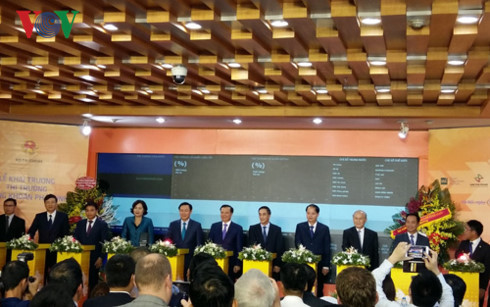
\includegraphics[scale=0.35]{fig1}
	\end{center}
	\label{reffig1}
\end{figure}
\begin{itemize}
	\item 10/08/2017: openning derivatives market \pause  %Vietnam has opened a derivatives market to draw more investment to its capital markets with future contracts 
	\item Derivative products: stock index and government bond futures \pause  %The market will initially start with two main derivative products and once fully operational, more instruments will be introduced.
	\item 12/2017: Options are expected to operate %
\end{itemize}	
\end{frame}

%------------------------------------------------

\begin{frame}
\frametitle{The potentiality of the barrier options}
\begin{block}{Barrier option}
	Barrier option is a type of option whose payoff depends on whether or not the underlying asset price has reached or exceeded some barrier level during the life of the option. %FPT current price 47, expected price is 55, barrier level is 42, knock-out, when the price down to 42, the option will be deactived.
\end{block} \pause
%The barrier options are popular and attractive thanks to benefits that they give investors more flexibility to express their view on the asset price movement in the option contract.
{\color{red}Advantages}
\begin{itemize}
	\item Matching beliefs about the future behavior of the market \pause
	\item Matching hedging needs more closely \pause
	\item Premiums are generally low %by not paying a premium to cover scenarios he or she views as unlikely
\end{itemize}
\end{frame}
%------------------------------------------------
\section{Methodology} %There are 2 method to derive European barrier call option: the partial differential equation approach and the martingale pricing(random probability) approach. We will use the martigale pricing approach.
\begin{frame}
%We may formulate the pricing models of barrier options using the martingale pricing approach and derive the corresponding price formulas by computing the expectation of the discounted terminal payoff.
\frametitle{The martingate pricing approach}
\begin{itemize}
	
	\item Based on the Black–Scholes pricing paradigm\pause \\[0.4cm]
	\item Using the reflection principle in the Brownian process\pause \\[0.4cm]% to obtain the transition density function
	\item Deriving the density function of the first passage time to the barrier %To compute the expected present value of the rebate payment
\end{itemize}
\end{frame}

\begin{frame}
\frametitle{New points}
\begin{figure}[htp]
	\begin{center}
		
\includegraphics[scale=.3]{fig2}
	\end{center}
	\label{reffig2}
\end{figure} \pause
\begin{itemize}
	\item Classifying some pricing formulas \pause 
	\item Applying FPT stock to the research formula
\end{itemize}
\end{frame}

\section{Objectives} 
\begin{frame}
\frametitle{Merits}
\begin{figure}[htp]
	\begin{center}
		
\includegraphics[scale=0.2]{fig3}
	\end{center}
	\label{reffig3}
\end{figure} \pause
	\begin{itemize}
		\item Applying the joint knowledge from 3 majors: risk management, finance and programming \pause
		\item Classifying the European barrier call option \pause
		\item Applying this formula for Vietnam derivative market, especially FPT stock
	\end{itemize}		
\end{frame}

\section{Process and Completion}
\begin{frame}
\frametitle{Completion}
	\begin{figure}[htp]
		\begin{center}
			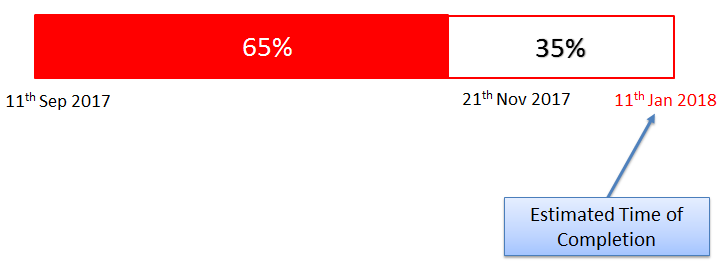
\includegraphics[scale=0.5]{fig4}
		\end{center}
		\label{reffig4}
	\end{figure} \pause
\begin{itemize}
	\item Completing 35\% report
	\item Deriving the Black-Scholes-Merton model
	\item Applying the Black-Scholes-Merton model to FPT stock
\end{itemize}
\end{frame}
\begin{frame}
	\frametitle{Remain tasks}
	\begin{itemize}
		\item Deriving the pricing model of the European barrier call option \\ [0.3cm]
		\item Apply this model to FPT stock \\ [0.3cm]
		\item Completing the report
	\end{itemize}
	
\end{frame}
\begin{frame}
\Huge{\centerline{\textcolor{red}{Thanks for listening}}}
\end{frame}
\end{document} 